\documentclass[12pt]{article}

% Language setting
% Replace `english' with e.g. `spanish' to change the document language
\usepackage[portuguese]{babel}

\usepackage{indentfirst}

% Set page size and margins
% Replace `letterpaper' with `a4paper' for UK/EU standard size
\usepackage[letterpaper,top=2cm,bottom=2cm,left=3cm,right=3cm,marginparwidth=1.75cm]{geometry}

% Useful packages
\usepackage{amsmath}
\usepackage{graphicx}
\graphicspath{ {./images/} }
\usepackage[colorlinks=true, allcolors=blue]{hyperref}


\title{Relatório do EP de MAC0209}
\author{André Luis Neves - 15493840\\Luis C. Vergara - 15472544\\Tiago de Souza Coelho - 15497994}

\begin{document}
\maketitle


\begin{abstract}
O trabalho  tem o objetivo de mostrar o efeito dos conceitos de precisão, acurácia, algarismos significativos e representação float sob a perspectiva da modelagem gráfica, ou seja, verificar as variações do modelo produzido devido a vários fatores, de forma experimental. 

\end{abstract}

\newpage

\tableofcontents

\newpage

\section{Introdução}

O trabalho foi desenvolvido com o intuito de aumentar a compreensão acerca da modelagem e das suas implicações no contexto das medições. Visto que uma medição sempre conterá erros, é necessário verificar como chegar a um equilíbrio entre um modelo com alta precisão e acurácia, sendo o mais simples possível, sob a ótica da navalha de Ockham.

Logo, sob uma perspectiva experimental, foi realizada essa experiência para compreender o que engloba a modelagem, em especial com respeito à modelagem matemática por meio de algoritmos computacionais.

Aqui são apresentadas as atividades desenvolvidas e seus resultados.

\section{Objetivos}

Esse trabalho visa analisar o erro de modelagem por meio da implementação de gráficos que refletem a precisão, acurácia, algarismos significativos e representação float, analisando os sinais de amostragem e quantização. Assim, pode ser dividido em 2 partes. A primeira é da análise do erro do gráficos por conta de sinais. A outra é comparar isso com valores teóricos conhecidos, como o Teorema da Amostragem de Nyquist-Shannon.

\section{Cronograma}

O trabalho foi começado no dia 04/03. Ele foi dividido em algumas etapas, as quais foram feitas em conjunto pelos membros do grupo.
As etapas foram, em ordem:

\begin{itemize}
\item Entender o problema e analisar o que e como deve ser resolvido. Prazo: 06/03

\item Escrever o código para plotar o gráfico. Prazo: 08/03

\item Escrever o código para plotar o erro absoluto. Prazo: 10/03

\item Escrever o código para salvar e carregar a planilha CSV. Prazo: 15/03

\item Ajustar o código, incluindo informações como legenda, nome dos eixos e título nos gráficos. Prazo: 18/03

\item Analisar as informações obtidas e escrever o relatório. Prazo: 26/03

\end{itemize}

\section{Dados e métodos}

Foram feitos os experimentos no trabalho:
\begin{itemize}

\item Plotar os gráficos de sin(x), log(x), atan(x)

\item Verificar o \textit{ground-truth} dos gráficos devido a diferentes taxas de amostragem

\item Verificar o \textit{ground-truth} dos gráficos devido a diferentes quantizações

\item Verificar o \textit{ground-truth} dos gráficos devido a salvamento e carregamento da planilha CSV

\end{itemize}

Os dados utilizados para plotar os gráficos foram a taxa de amostragem e a de quantização. Elas são os únicos dados que mudam de um gráfico para o outro.

Para tanto, foram usadas as bibliotecas \textit{matplotlib} para plotar os gráficos e \textit{pandas}, \textit{numpy} para salvar e carregar dados da planilha CSV. Os métodos específicos e implementações estão disponíveis no JN enviado, devidamente comentados e explicados.

\section{Resultados experimentais}

\begin{figure}[h]
    \centering
    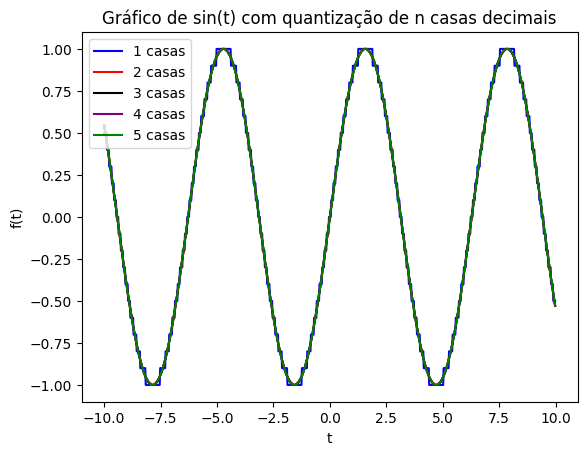
\includegraphics[width=0.5\linewidth]{sin_amostragem.png}
    \label{fig:enter-label}
\end{figure}

\begin{figure}[h]
    \centering
    \includegraphics[width=0.5\linewidth]{log_amostragem.png}
    \label{fig:enter-label}
\end{figure}

\clearpage

\begin{figure}[h]
    \centering
    \includegraphics[width=0.5\linewidth]{atan_amostragem.png}
    \label{fig:enter-label}
\end{figure}

Os gráficos acima corroboram com o Teorema da Amostragem de Nyquist-Shannon, já que temos: para uma amostragem suficientemente grande, ou seja, para $f_\text{s} >= f_\text{máx}$, onde $f_\text{máx}$ é a frequência dos valores do gráfico (dizemos $(\frac{1}{\Delta t} \approx \frac{1}{dt})$)

\begin{figure}[h]
    \centering
    \includegraphics[width=0.5\linewidth]{sin_quant.png}
    \label{fig:enter-label}
\end{figure}

\clearpage

\begin{figure}[h]
    \centering
    \includegraphics[width=0.5\linewidth]{cos_quant.png}
    \label{fig:enter-label}
\end{figure}

\begin{figure}[h]
    \centering
    \includegraphics[width=0.5\linewidth]{atan_quant.png}
    \label{fig:enter-label}
\end{figure}

Nos gráficos quantizados, é possível observar um certo erro para até 1 casa decimal. Mas, abaixo disso, os gráficos se sobrepõe completamente, até mesmo não sendo possível ver os de 2, 3, 4 e casas decimais. Assim, se revela esperado, pois taxa de erro é $<= 5 * 10^\text{-n}$ para uma quantização de n casas decimais. Esse resultado se reflete no erro absoluto encontrado para as funções. Tomamos como exemplo as duas a seguir:

\clearpage

\begin{figure}[h]
    \centering
    \includegraphics[width=0.5\linewidth]{sin_2casas.png}
    \label{fig:enter-label}
\end{figure}

\begin{figure}[h]
    \centering
    \includegraphics[width=0.5\linewidth]{log_4casas.png}
    \label{fig:enter-label}
\end{figure}

Além disso, temos que o erro devido à salvar uma planilha CSV existe, mas é quase desprezível, uma vez que é da ordem de $10^\text{-16}$, conforme imagens abaixo:


\begin{figure}[h]
    \centering
    \includegraphics[width=0.5\linewidth]{sin_csv.png}
    \label{fig:enter-label}
\end{figure}

\begin{figure}[h]
    \centering
    \includegraphics[width=0.5\linewidth]{cos_csv.png}
    \label{fig:enter-label}
\end{figure}

\begin{figure}[h]
    \centering
    \includegraphics[width=0.5\linewidth]{atan_csv.png}
    \label{fig:enter-label}
\end{figure}

\clearpage

\section{Discussão e Conclusão}
Aplicamos o teorema de Nyquist-Shannon ao escolher nossa frequência para amostragem para evitar aliasing durante a interpolação do sinal de tempo discreto, e verificamos o teorema obtendo uma nova função com uma frequência não menor que o sinal de tempo contínuo original.
Embora as três funções fossem simples, as funções seno, log e arctan são representativas de sinais da vida real, e nos permitem aplicar a quantização e o teorema de Nyquist-Shannon de forma controlada.

\end{document}

